% 1. Introdução
\chapter{Introdução}

A linguagem de programação C \cite{CLANG} é a fundação de programação de sistemas. Até a incorporação de Rust no começo de 2024 \cite{RUSTFORLINUX}, C era a única linguagem do \emph{kernel} do Linux. Mesmo com essa grande importância, C é extremamente vulnerável a falhas de memória, com muito poucas restrições do compilador a fim de evitar essas falhas. Essa liberdade é, em parte, o ponto da linguagem C, que serve como uma simples fachada genérica sobre o Assembly da máquina. Porém, C faz parte de muitas partes críticas de infraestrutura para que a validação de novos sistemas não seja feita de forma rigorosa. 

No começo do milênio, Cyclone \cite{CYCLONE1} começou a popularizar linguagens de programação de baixo nível com sistema de memória seguro sem o uso amplo de \emph{Garbage Collectors} (GC). Essa tendência foi seguida,alguns anos depois, pelo projeto da Microsoft, CCured \cite{CCURED}. Essas duas linguagens partiram da sintaxe de C e adicionaram elementos de segurança de memória, com o fim de facilitar o porte de programas em C para essa versão com mais ferramentas de segurança.

No começo dos 2010s, o projeto Rust \cite{RUSTBOOK} surgiu com novas propostas de solução de memória, quebrando o paradigma da similaridade com C. Essas novas técnicas, principalmente o \emph{Borrow Checker}, apresentaram oportunidades de segurança sem perda de desempenho, coisa que os seus predecessores não conseguiram atingir. A partir disso, novos sistemas foram emergindo, partindo de novas tecnologias como LLVM \cite{LLVM} que simplificam o processo de desenvolvimento de linguagens de programação, cada uma com uma proposta nova de como evitar falhas de memória.

O ambiente rico em soluções de segurança de memória evoca o pensamento: quais são corretas? Quais são efetivas? Quais tornam a linguagem restrita? Para linguagens que pretendem ser posicionadas em caminhos críticos de infraestrutura, como Rust, a demonstração de sua corretude é fundamental para a sua adoção e a possibilidade de se concorrer com o atual déspota de sistemas de baixo nível, C.

\section{Trabalhos Relacionados}


Muitos dos trabalhos de prova de solução de memória focam na linguagem Rust e seu \emph{Borrow Checker}. O projeto RustBelt \cite{RUSTBELT}, fundado em 2017, tinha como meta provar a corretude do \emph{Borrow Checker} de Rust e do seu sistema de tipos. Para isso, é utilizada uma versão de Rust formulada em \emph{continuation-passing style} para gerar os sistemas de prova. O sistema de detecção de falhas desse projeto inspirou o sistema de $PCL_{back}$ (\emph{back-end Porcelain}). Uma alternativa a esse projeto foi \emph{Sound Borrow-Checking for Rust via Symbolic Semantics} \cite{RUSTSYMBOLIC}. Nele, realiza-se um método de prova similar ao almejado neste trabalho, de realizar provas sobre a compilação de um programa para uma linguagem-base. A definição de $PCL_{front}$ foi baseada no algoritmo do Polonius \cite{Stjerna1684081}, entretanto, outras formulações desses foram construídas e provadas corretas, como \emph{A Lightweight Formalism for Reference Lifetimes and Borrowing in Rust} \cite{RUSTFORMALISM}. 

%	1.3 Objetivos
\section{Objetivos}

O objetivo desse projeto é a construção de um framework formal, denominado Porcelain,  que expõe as falhas de memória que ocorrem durante a execução de programas e permite provar a ausência de tais falhas como consequência da introdução de certas técnicas de segurança de memória. Os principais componentes de Porcelain podem ser observados na Figura~\ref{fig:pcl:framework}. Neste, temos uma linguagem similar a C denominada $PCL_{back}$ (back-end Porcelain), instrumentada para detectar e classificar falhas de memória. Também temos uma linguagem que compilará para a linguagem base, $PCL_{front}$ (\emph{front-end Porcelain}), a qual terá um sistema de análise estática, similar ao sistema de \emph{Borrow Checker} de Rust, incorporado às regras de seu sistema de tipos. Dado que todos esses elementos serão formalmente definidos, espera-se tornar possível a garantia de ausência de certas falhas em memória para a execução (em $PCL_{back}$) de programas obtidos através da compilação de programas  $PCL_{front}$ bem tipados, através de técnicas tais como indução estrutural nas derivações de tipos. 


\begin{figure*}[ht]
	\caption{Componentes do framework Porcelain}
	\label{fig:pcl:framework}
	\begin{center}
    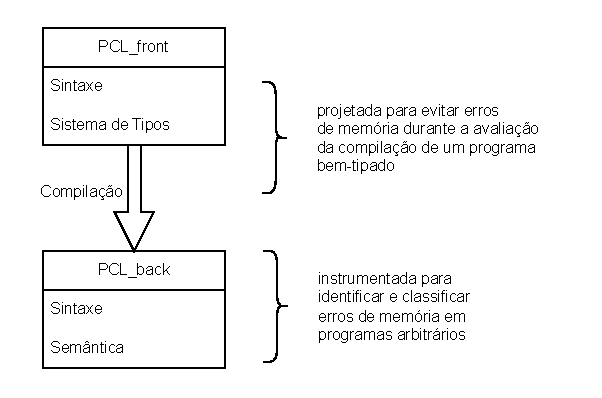
\includegraphics[scale=0.9]{figures/pcl.drawio.pdf}
    \end{center}
	\legend{Fonte: Os Autores.}
\end{figure*}



Este trabalho contribui para a discussão de falhas de memória e serve como um meio flexível de provar outras estratégias não convencionais em um campo mais neutro. Dessa forma, ele permite estratégias \emph{bottom-up} no desenvolvimento de linguagens, em que primeiro decide-se e prova-se uma estratégia de memória, para depois desenvolver a linguagem que a envolve.

%	1.4 Organização
\section{Organização}

O restante deste trabalho é organizado da seguinte forma: no Capítulo \ref{chap2} são elaborados conceitos básicos para o entendimento do projeto. Isso inclui uma explicação simples de semântica operacional e sistema de tipos, junto de uma elaboração sobre falhas de memória: significado, tipos e soluções propostas ao longo dos anos. No Capítulo \ref{chap3} é introduzido $PCL_{back}$, a linguagem-alvo de compilação do projeto. Para isso, elabora-se sobre as suas estruturas de avaliação, regras e correspondência com os erros do capítulo \ref{chap2}. Com esses dois capítulos, define-se a base do projeto. A partir desse ponto, passa-se a discorrer um caso de uso do sistema. O Capítulo \ref{chap4} discorre sobre os conceitos necessários para o desenvolvimento da linguagem $PCL_{front}$, explicada no Capítulo \ref{chap5}. O projeto é concluído pelo Capítulo \ref{chap7}.
